\documentclass[border=15pt]{standalone}
\usepackage{amsmath,amssymb,mathtools}
\usepackage{tikz}
\usepackage{pgfplots}
\usepackage{pgf}
\begin{document}
	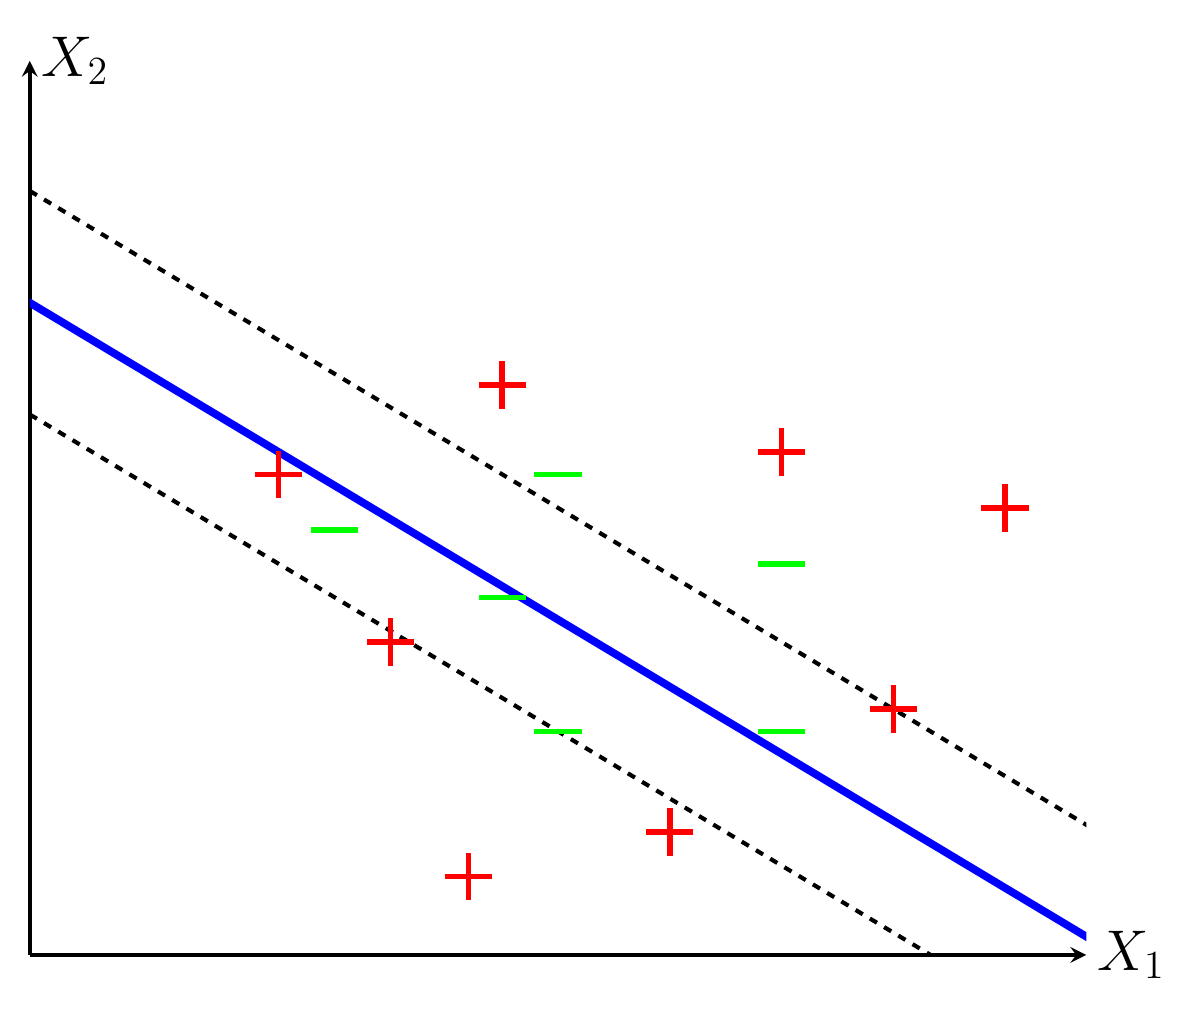
\begin{tikzpicture}
		\begin{axis}[
			xmin=1,
			xmax=9,
			ymin=1,
			ymax=9,
			axis equal,
			width=15cm,
			axis x line=center,
			axis y line=center,
			xmajorticks=false,
			ymajorticks=false,
			ylabel style={right,font=\huge},
			ylabel=$X_2$,
			xlabel style={above,right,font=\huge},
			xlabel=$X_1$,
			line width=1.5pt
			]
			%\addplot[no markers, domain=-1:11]{(5/3)*x};
			
			\addplot[only marks, mark=-,draw=green,mark size=0.3cm,line width=2pt]coordinates {(5,3) (4.5,4.2) (5,5.3) (3,4.8) (7,3) (7,4.5)};
			\addplot[only marks, mark=+,draw=red,mark size=0.3cm,line width=2pt]coordinates {(8,3.2) (4.5,6.1) (7,5.5) (6,2.1) (4.2,1.7) (3.5,3.8) (2.5,5.3) (9,5)};
			\addplot[no markers,domain=-1:11,thick,blue,line width=2.8pt]{-0.6*x+7};
			\addplot[no markers, domain=-1:11,dashed,line width=1.5pt]{-0.6*x+8};
			\addplot[no markers, domain=-1:11,dashed,line width=1.5pt]{-0.6*x+6};
		\end{axis}
	\end{tikzpicture}
\end{document}